\documentclass[a4paper, 12pt]{article}
\usepackage[T1]{fontenc}
\usepackage[scale=1,angle=0,opacity=1,color=black!60]{background}
\usepackage{tikzpagenodes}
\usepackage{lastpage}
\usepackage{lmodern}
\usepackage{float}
\usepackage{adjustbox}
\usepackage{amsmath}
\usepackage{nccmath}
\usepackage{url}
\usepackage{listings}
\usepackage{alltt}
\usepackage[section]{placeins}
\usepackage{tocloft}
\renewcommand{\cftsecleader}{\cftdotfill{\cftdotsep}}  % lineas punteadas en la tabla de contenidos
%\newcommand\mydotfill{\cftdotfill{\cftdotsep}}

\usepackage[textwidth=420pt,textheight=630pt]{geometry}
\setlength{\oddsidemargin}{15.5pt}
%\usepackage[none]{hyphenat} %no cortar palabras

\usepackage[spanish, activeacute]{babel} %Definir idioma español
\usepackage[utf8]{inputenc} %Codificacion utf-8
\backgroundsetup{contents={}} %Saca el 'draft'
\definecolor{mygray}{rgb}{0.95,0.95,0.95}

\usepackage{listings}
\lstset{
    basicstyle=\footnotesize,
    backgroundcolor=\color{mygray},
    breaklines=true,
    breakatwhitespace=true,
    postbreak=\mbox{\textcolor{red}{$\hookrightarrow$}\space},
    captionpos=b,
    keepspaces=true,
    numbers=left,
    numbersep=5pt,
    showspaces=false,
    showstringspaces=false,
    showtabs=false,
    tabsize=4,
    language=C,
    frame=none,
	title=\lstname,
}

\def\labelitemi{$\bullet$}

\begin{document}
	% TÍTULO, AUTORES Y FECHA
	\begin{titlepage}
		\vspace*{\fill}
		\begin{center}
			\Large 75.10 Tecnicas de diseño \\
			\Huge Trabajo Práctico 1: validador de ofertas \\
			\textbf{Fecha de Entrega:} 3/10/2018\\
			\bigskip
			\begin{center}
				\begin{tabular}{||c | c||} 
					\hline
					Integrantes & Padron \\ [0.5ex] 
					\hline\hline
					Augusto Arturi & 9.... \\
					\hline
					Pablo inoriza & 9.... \\
					\hline
					Manuel, Llauro & 9.... \\
					\hline
					Sebastián Ezequiel Blanco & 98539 \\
					\hline
				\end{tabular}
			\end{center}

		\end{center}
		\vspace*{\fill}
	\end{titlepage}
	\pagenumbering{arabic}
	\newpage

	% ÍNDICE
	\tableofcontents
	\newpage
	\pagenumbering{arabic}

	\section{Modelo del dominio}
		\begin{figure}[ht]
			\begin{adjustbox}{addcode={
				\begin{minipage}{\width}}{
					\caption{%
						Modelo del dominio
						}
				\end{minipage}},rotate=360,center}
				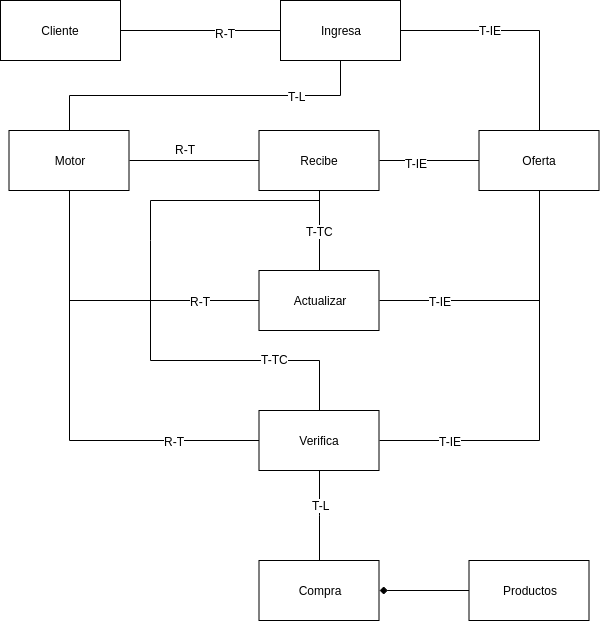
\includegraphics[scale=.6]{ModeloDominio.png}
			\end{adjustbox}
		\end{figure}
		\FloatBarrier
		\newpage

	\section{Explicacion de los modulos}
		% OFFER_PROCESSOR	
		\subsection{offer\_processor}
			Este modulo es el principal del trabajo y contiene la interfaz publica que se provee al usuario, donde exiten dos 				funciones:\\
			\begin{lstlisting}[frame=tb, caption=firmas de la interfaz publica, label=zebra, tabsize=1]
				[state] initialize-offers [offers rules]
				[offers-applied] = process-sale [state, sale]
			\end{lstlisting}
			La primer funcion (initialize-offers) recibe una lista de ofertas y una lista de reglas y las almacena retornando un 				valor que representa una estado. \\
			La segunda funcion (process-sale) recibe el estado que se obtubo de la funcion anterior y recibe una compra que 			contiene productos, un calendario y una forma de pago, retornando un vector donde cada elemneto representa una oferta 				que aplico a la compra con el respectivo descuento.
		
		\newpage
		% OFFER_APPLIER
		\subsection{offer\_applier}
			Este modulo tiene una sola funcion que obra de interfaz publica y es la siguiente:
			\begin{lstlisting}[frame=tb, caption=firmas de la interfaz publica, label=zebra, tabsize=1]
				[offers-applied] = apply_offer [offer sale]
			\end{lstlisting}
			Esta funcion recibe una unica oferta se la aplica a la respectiva compra (sale) retornando un vector de mapas donde 				cada uno tiene el sigueinte formato:
			\begin{lstlisting}[frame=tb, caption=mapa resultado de ofertas aplicadas, label=zebra, tabsize=1]
				{
					"description" "una descripcion"
					"offer_code" "un codigo"
					"discount" "un valor"
				}
			\end{lstlisting}
			Cada oferta tiene un porcentaje de descuento y una compra tiene varios productos, por lo tanto en cada uno de estos 				mapas $"discount"$ es el valor que se descuenta por cada producto que cumple con la oferta.\\
			Luego tenemos funciones internas del modulo que resuelven otros porblemas y las firmas son estas:
			\begin{lstlisting}[frame=tb, caption=firmas de las funciones privadas, label=zebra, tabsize=1]
				[products] get_products_that_met_the_rules [offer sale]
				[offers-applied] get_offer_result [offer products]
				[discount-value] apply_discount [offer price]
			\end{lstlisting}
			La primer funcion recibe una oferta y una compra y retorna una lista de productos los cuales cumplen con la oferta.
			Cada producto de este vector que retorna tiene un formato nuevo con un criterio propio. el formato de cada producto es 				cambiado dentro de esta funcion para facilitar el diseño del codigo y con un ejemplo mostramos como representamos un 				producto:
			\begin{lstlisting}[frame=tb, caption=formato de un producto, label=zebra, tabsize=1]
				{
					'products' {
						'name' 'Leche Descremada 1L, la Calmisima'
						'brand' { 
							'code' 'Z001ABC' 
							'name' 'La Calmisima' 
						}
						'category' { 
							'code' 'X033AXX' 
							'name' 'Lacteo' 
						}
						'price'  25.40
						'iva_porcentage' 10.5
						'code' 'X033XXX'
					}
					'payment' { 
						'method' 'CASH' 
						'bank' 'CAPRO' 
					}
					'purchase_date' {
						'year' '2018'
						'month' 'SEPTEMBER'
						'day_number' 20
						'week_day' 'Thursday'
						'week_number' 4
					}
				}
			\end{lstlisting}
			La segunda funcion (get\_offer\_result) recibe una oferta y una lista de productos (con el formato ya explicado) que 				cumplen con dicha oferta y retorna un vector de oferta aplicadas cuyo formato de cada oferta aplicada se explico 				anteriormente (ver Listing 3: mapa resultado de ofertas aplicadas).
		
		\newpage
		% RULE_APPLIER
		\subsection{rule\_applier}
			Este modulo tiene una sola funcion que obra de interfaz publica y es la siguiente:
			\begin{lstlisting}[frame=tb, caption=firmas de la interfaz publica, label=zebra, tabsize=1]
				[boolean-vector] = apply_rules [rules_codes prod]
			\end{lstlisting}
			Esta funcion recibe un vector de codigos de relgas y un producto con un formato explicado anteriormente 
			(ver Listing 5: formato de un producto) y retorna un vector de boleano donde cada uno representa si el producto cumple 				o no con cada regla (true: cumple, false: no cumple).\\
			
			Luego tenemos funciones internas del modulo que resuelven otros porblemas y las firmas son estas:
			\begin{lstlisting}[frame=tb, caption=firmas de las funciones privadas, label=zebra, tabsize=1]
				[rule] get_rule [rule_code]
				[boolean] atomic_rule [rule prod]
				[boolean] apply_atomic_rule [rule prod]
				[boolean-vector] multiple_rules [rules_codes prod]
				[boolean-vector] apply_multiple_rules [rules_codes prod]
			\end{lstlisting}
			La primer funcion (get\_rule) recibe el codigo de una regla y devuelve la regla.\\
			La segunda funcion (atomic\_rule) es un multimetodo el cual recibe una regla y un producto con un formato explicado 				anteriormente (ver Listing 5: formato de un producto) y devuelve un booleano que nos dice si el producto cumple o no 				con la regla. Esto es un multimetodo ya que no sabemos si la regla es atomica o es una regla con subreglas, por lo tanto
			si la regla es atomica ejecuta la funcion apply\_atomic\_rule, la cual recibe una regla atomica y un producto y retorna 			un boleano. Si la regla no es atomica llama a otro multimetodo que es multiple\_rules, que recibe una regla no atomica 				y el producto. Si la regla no atomica esta compuesta por una unica subregla ejecuta apply\_atomic\_rule donde recbe la 				subregla y el producto. Si la regla no atomica esta compuesta por mas de una subregla ejecuta apply\_multiple\_rules 				donde recibe un vector de codigos de subreglas y el producto y retonra un vector de booleanos.

		\newpage
		% INSERTIONS
		\subsection{insertions}
			Este modulo tiene dos funciones que obran de interfaz publica y son las siguientes:
			\begin{lstlisting}[frame=tb, caption=firmas de la interfaz publica, label=zebra, tabsize=1]
				[nil] add_offer [o]
				[nil] add_rule [r]
			\end{lstlisting}
			La primer funcion recibe un vector de ofertas y lo almacena en una variable global llamada offers\_vector. Dentro de la 			funcion hace chequeos de datos y en caso de haber un dato invalido retorna excepcion.\\
			La segunda funcion recibe un vector de reglas y lo almacena en una variable global llamada rules\_vector. dentro de la 				funcion hace chequeos de datos y en caso de haber un dato invalido retorna excepcion.\\
		\newpage
		% OPERATORS
		\subsection{operators}
			Este modulo tiene una funcion que obra de interfaz publica y es un multimetodo y es la siguiente:
			\begin{lstlisting}[frame=tb, caption=firmas de la interfaz publica, label=zebra, tabsize=1]
				[boolean] apply_op [op values field]
			\end{lstlisting}
			Esta funcion recibe un string (op) que representa la operacion a realizar y dependiendo que tipo de operacion values 
			y/o field tomas distintos formatos. Si se quiere ejecutar las operaciones AND, OR, NOT , values sera un vector de 				boleanos al cual de le apicara dicha operacion y field sera nil, ya que no se usara. Si se quiere ejecutar las 				operaciones LOWER, HIGHER, EQUALS values sera un valor singular y field tambien. Si se quiere ejecutar la operacion IN, 			values sera un vector de valores y field sera un valor singular.

		\newpage
		% FIELDS
		\subsection{fields}
			Este modulo tiene una sola funcion que obra de interfaz publica y es la siguiente:
			\begin{lstlisting}[frame=tb, caption=firmas de la interfaz publica, label=zebra, tabsize=1]
				[field] get_field [product rule]
			\end{lstlisting}
			Esta funcion recibe un producto	con un formato explicado anteriormente (ver Listing 5: formato de un producto) y una 				regla y retorna el campo del producto el cual la regla especifica.\\

			Luego tenemos funciones internas del modulo que resuelven otros porblemas y las firmas son estas:
			\begin{lstlisting}[frame=tb, caption=firmas de las funciones privadas, label=zebra, tabsize=1]
				[path] rule_field_path [rule]
				[key] translate [value])
			\end{lstlisting}
			La primer funcion recibe una regla y retorna un vector de claves de un mapa en el cual se encuetra el valor buscar en 				el producto.\\
			La segunda funcion es un multimetodo y recibe una clave que representa parte del camino (path) para encontrar el field 				y lo traduce a el nombre que el mapa usa, ya que por ejemplo las reglas usan la palabra CALENDAR para referirse al 				campo purchase\_date de un producto.		

		\newpage
		% EXCEPTIONS
		\subsection{exceptions}
			Este modulo tiene cuatro funciones que obran de interfaz publica que son multimetodos y son las siguientes:
			\begin{lstlisting}[frame=tb, caption=firmas de la interfaz publica, label=zebra, tabsize=1]
				[field/Exception] check_field [field msg]
				[id/Exception] check_unknown_id [id]
				[rules/Exception] check_cycle_id [rules]
				[ids/Exception] check_duplicate_codes [ids code]
			\end{lstlisting}
			La primer funcion recibe un campo y un mensaje y si dicho campo es invalido, es decir tiene un valor que no esta 				permitido, retorna una excepcion con el mensage. En caso contrario retorna el campo.\\
			La segunda funcion recibe un id que puede estar en formato json o no y si no contiene ningun dato o es un nill retorna 				excepcion. En caso contrario retorna el id.\\
			La segunda funcion recibe un vector de reglas y si existen reglas no atomicas las cuales son ciclicas retorna una 				excepcion. En caso contrario retorna las reglas.\\
			La segunda funcion recibe un vector ids que podrian ser tanto reglas como ofertas y si existen dos id con el campo code 			en el mismo valor retirna excepcion. En caso contrario retorna las reglas.\\

		\newpage
		% CONVERTIONS
		\subsection{convertions}
			Este modulo tiene dos funciones que obran de interfaz publica y son las siguientes:
			\begin{lstlisting}[frame=tb, caption=firmas de la interfaz publica, label=zebra, tabsize=1]
				[structure] json_to_map [j]
				[json] map_to_json [j] 
			\end{lstlisting}
			La primera funcion recibe un string (json) y lo retorna en la estructura de datos correspondiente de clojure.\\
			La segunda funcion recibe una estructura de datos clojure y la convierte en string (json).\\

		\newpage
		% TRANSLATIONS
		\subsection{translations}
			Este modulo tiene una sola funcion que obra de interfaz publica que es un multimetodo y es la siguiente:
			\begin{lstlisting}[frame=tb, caption=firmas de la interfaz publica, label=zebra, tabsize=1]
				[month] translate [month]
			\end{lstlisting}
			Esta funcion recibe un mes en español o ingles y lo retorna en español. Esto se debe a que la veces se termina 				comparando los mismos meses en distintos idiomas y la comparacion da falso, por lo tanto  no aseguramos de tener todo 				en un mismo idioma.
			
\end{document}
